\chapter{Soluciones coloidales}

%%%%%%%%%%%%%%%%%%%%%%%%%%%%%%%%%%%%%%%%%%%%%%%%%%
\section{Introducci\'on}

En los \'ultimos cap\'itulos, hemos hecho hincapi\'e en la importancia y el potencial uso de los geles polim\'ericos. Nos hemos enfocado especialmente en su aplicaci\'on para el secuestro de prote\'inas y/o f\'armacos de inter\'es terap\'eutico.
En este sentido, en los dos \'ultimos cap\'itulos hemos presentado dos tipos de modelos que permiten estudiar la fisicoqu\'imica de un nano/microgel aislado en soluci\'on.
En el cap\'itulo  \ref{Chapter-geles} hemos hecho referencia a un modelo robusto en el cual se ha modelado el sistema como uno de dos fases con el cual logramos explicar la respuesta de los microgeles con respuesta a  m\'ultiples est\'imulos. Como los cambios en pH, temperatura o concetraci\'on de sal afectan a la capacidad de adsorber y liberar distintas moleculas, as\'i como sus cambios de tama\~no y carga. 
En el siguiente cap\'itulo,\ref{Chapter-esfericas} , hemos complejizado nuestro modelo para investigar c\'omo la estructura interna afecta la respuesta de estos geles. Así como la obtención de información que no era accesible con el modelo anterior: localización de la adsorci\'on y reordenamiendo de la estructura interna de los geles debido a est\'imulos externos.
Con el modelado propuesto en este cap\'itulo  se ha podido  demostrar  que el dise\~no de la estructura de los nanogeles,  pensar en distintas estrateg\'ias de  s\'intesis, son factores importantes para optimizar los procesos de encapsulaci\'on y liberaci\'on de prote\'inas. 
Para poder acercanos más a los modelos experimentales damos un paso hacia las soluciones de nanogeles, las cuales son las que se utilizan para el desarrolo tecnologico que nos proporcionan estos sistemas polim\'ericos.

En este \'ultimo cap\'itulo,  indagaremos la fisicoqu\'imica de las soluciones de nanogeles. Como se ven afectados los comportamientos individuales, ya reportados en los cap\'itulos anteriores, ahora en funci\'on de la cantidad de ellos en soluci\'on, su concentraci\'on.
En esta primera aproximaci\'on usamos como m\'etodo de estudio simulaciones del tipo MonteCarlo y como referencia se utiliza el modelo y teor\'ia del sistema de dos fases presentado en el cap\'itulo \ref{Chapter-geles}. La combinaci'on de estos estudios nos permite tener informaci\'on que logra explicar comportamientos reportados experimentalmente como lo son ...
\textcolor{red}{agregar citas de algunos resultados experimentales}



Estudio sobre las soluciones coloidales de nanogeles polimericos....

\section{M\'etodo: Simulaci\'on Monte Carlo}


La simulaci\'on de sistemas de nanogeles en soluci\'on es una herramienta invaluable para comprender su comportamiento y sus propiedades termodin\'amicas. En este estudio, se emple\'o el m\'etodo Monte Carlo, en particular el algoritmo de Metropolis-Monte Carlo, para modelar la soluci\'on de nanogeles.
El m\'etodo de Metropolis-Monte Carlo se fundamenta en la generaci\'on aleatoria de n\'umeros y la evaluaci\'on de distintos estados o configuraciones del sistema en estudio. En cada paso de la simulaci\'on, se selecciona de manera aleatoria una configuraci\'on y se calcula su energ\'ia o probabilidad seg\'un un modelo predefinido que describe las interacciones entre las part\'iculas de nanogeles y el solvente.
La simulaci\'on Monte Carlo, mediante el algoritmo de Metropolis-Monte Carlo, ofrece una perspectiva \'unica para explorar las propiedades de los nanogeles en soluci\'on y su comportamiento en diferentes condiciones. 
En el caso espec\'ifico de nuestra soluci\'on de nanogeles, una configuraci\'on consiste en el movimiento y aumento de tama\~no de una part\'icula (nanogel) seleccionada al azar. 
En este sentido la probabilidad de acetar o no dichos cambios en el sistema biene dado por:

\begin{align}
	P(s) = min \{e^{-(\Delta U^s_{inter} + \Delta U^s_{intra})},1\}
\end{align}

En donde $P(s)$ indica la probabilidad de aceptaci\'on del estado $s$, como mencionamos este consta de un cambio en el tama\~no y posici\'on de una nanogel. $\Delta U^s_{intra}$ corresponde al cambio en la energ\'ia interna de cada nanogel, debido a un cambio en su tama\~no, la energ\'ia de estos estados es obtenida usando una teor\'ia termodin\'amica detallada en el cap\'itulo  \ref{Chapter-geles}. Como moestramos en ese cap\'itulo el modelo de dos fases nos permite obtener la informaci\'on termodin\'amica necesarioa para explicar el comportamiento de una nanogel aislado.
El costo energetico de adsorber solvente, con sus respectivo iones, energ\'ia el\'astica... 
Por otro lado la energ\'ia intermolecular, $\Delta U_{inter}$, viene dada por la interacci\'ion de a pares de todos los nanogeles en soluci\'on. 
Para esta interacci\'on de a pares se ha utilizado un potencial combinado: Hertz-Yukawa. Este potencial fue previamente utilzado en \addcite[weyer2018concentration], en los cuales \addcite[weyer2018concentration] 
estudiaron la hinchaz\'on y las propiedades estructurales de suspensiones de microgeles i\'onicos su teor\'ia inlcuye las interacciones el\'asticas efectivas de Hertz y una teor\'ia de interacciones electrost\'aticas efectivas dependientes de la densidad (Yukawa). 
(un poco m\'as de los potenciales)
\textcolor{red}{Porque los podemos usar para nuestro sistema..}
Estamos trabajamos con materiales blandos que son deformables, por tando es posible modelarlos usando un potencial de Hertz, en el cual se considera la superposici\'on de las part\'iculas involucradas.
Yukawa por su parte es un potencial del tipo columbico mediado por el medio dilectrico en el que se encuentra. Se ven involucradas las cargas que envuelven a cada nanogel considerando la longitud de Debye. 
Podemos resumir nuestro potencial total de trabajo como:

\begin{align}
	U_{inter}(r) = \begin{cases} U_H + U_Y & \text{if } r \leq a_i + a_j \\ U_Y & \text{if } r > a_i + a_j \end{cases} 
	\label{eq:HY-potential}
\end{align}

en donde $r$ es la distancia entre dos nanogeles, definida como la distancia de sus centros. 
$a_i$ y $a_j$ representan los radios de el nanogel $i$ y $j$ respectivamente. Por ello la condici\'on $r \leq a_i +a_j$ representa la superposici\'on de estas particulas, deformandose y entrando en juego el potencial de Hertz.
Para mayores distancia a la suma de los radios de cada nanogel se pone en juego el potencial de Yukawa. Para el cual se define:
\begin{align}
	\beta u_Y(r) = q_i q_j \frac{e^{\kappa(a_i + a_j)}}{(1 +\kappa a_i)(1 + \kappa a_j)} \frac{e^{-\kappa r}}{r} 
	\label{eq:yukawa}
\end{align}

En donde $q_i$ y $q_j$ son las cargas netas que poseen los nanogeles $i$ y $j$ respectivamente. El valor $\kappa$ corresponde a la constante de apantallamiento de Debye. 
El pontecial de Hertz, $U_H$, se define como:
 

\begin{align}
	\begin{aligned}
		& \beta u_H (r) = \left(\frac{1-r}{a_i + a_j}\right)^{5/2}\times b_{12} \\
	\end{aligned}
\end{align}


En donde $b_{12}$ es la constante de interacci\'on entre las part\'iculas la cual depende de las propiedades el\'asticas del nanogel a trav\'es del m\'odulo de Young $\Lambda$ y el radio de Poisson $\nu$. \addcite[landau] La teor\'ia de escalado en sistemas de redes polim\'ericas predice que en buenos solventes \addcite que el m\'odulo de Young  escala linealmente con la temperatura y la densidad de los entrecruzamientos (o n\'umero de cadenas): $\Lambda \approx TN_{ch}/v$. Cuanto m\'as densos sean los entrecruzamientos, m\'as r\'igido ser\'a el gel.
Con lo cual podemos definir $b_{12}^\ast = \beta b_{12}$ el cual nos independiza de la temperatura y solo tenemos la dependencia con el n\'umero de cadenas ($N_{ch}$) y grado de entrecruzamiento de nuestro nanogel. 


\section{Resultados}


\begin{figure*}[!tb]
	\centering
	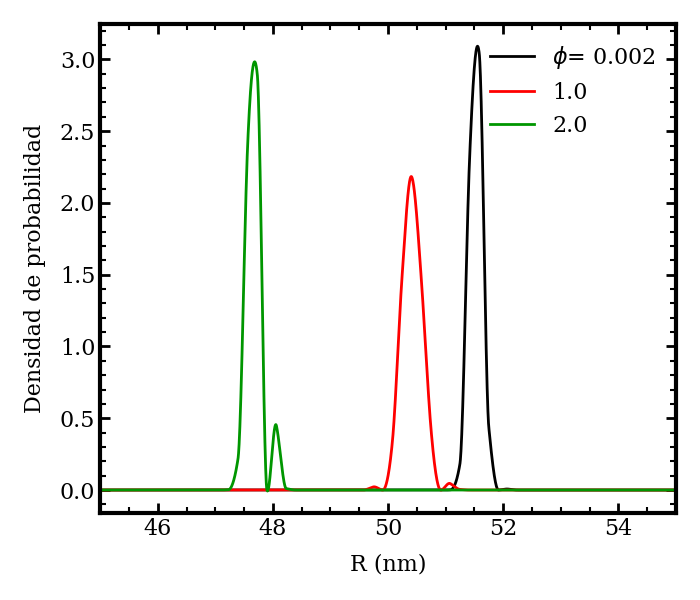
\includegraphics[width=1\linewidth]{Figures/graph-mc/sizes.png}
	\caption{Gr\'afico del probabilidad de tama\~no de la soluci\'on de  nanogeles en funci\'on de la densidad... fracci\'on de volumen ocupada.}
	\label{fig:mc:sizes-phi}
\end{figure*}

